\documentclass[fleqn,10pt]{wlscirep}
\usepackage[utf8]{inputenc}
\usepackage[T1]{fontenc}
\usepackage{bm}
\title{Nature Reviews Materials title with no punctuation and no more than 90 characters}

\author[1,*]{Author1 Name Surname}
\author[2]{Author2 Name Surname}
\author[1,2]{Author3 Name Surname}
\author[2]{Author4 Name Surname}
\affil[1]{Affiliation, Department, City, Country}
\affil[2]{Affiliation, Department, City, Country}

\affil[*]{e-mail: name.surname@email.edu}


\begin{abstract}
About 150 words. This is a taster of the article to get the reader to read on rather than a standard abstract so does not need to be very detailed. You should include some key words to improve article discovery in online searches but avoid using specialist jargon so as not to alienate general readers. Here are some difference.

Let's do something new.
This is hard but fun hhh.
Let's try something else!

Let's try some Chinese! Wow that's really fun bro!

This is a little bit hard for me but I think I'm enjoy it. Let finish it!

See some fork things.
\end{abstract}
\begin{document}

\flushbottom
\maketitle

\thispagestyle{empty}

\section*{Main text}

Total text of article 6,000–8,000 words (i.e. from the Introduction to the Outlook section; without including the abstract, figure captions or text boxes).



\section*{Introduction}

We recommend that you keep the introduction to 800 words maximum. The introduction should answer the following questions: what is the topic of the article? Why is this topic of importance? What recent developments make it timely to review this topic now? And how will this topic be reviewed? To answer the last question, we recommend adding a guiding paragraph at the end of your introduction that clearly states what will (and what won’t) be discussed in your Review, so readers and referees will know what to expect.


\section*{Main text heading 1}

Please use headings/subheadings to break up the text. Main headings should be no more than 38 characters, including spaces.

\subsection*{Subheading 1}

Subheadings should be no more than 39 characters, including spaces. In the final layout, subheadings will be in-line and thus followed by a full stop.

\subsubsection*{Second-level subheading 1}
Second-level subheadings should be no more than 70 characters, including spaces.

\section*{Main text heading 2}

\subsection*{Subheading 2}
\subsubsection*{Second-level subheading 2}
...\\
...

\section*{Outlook/Future Perspectives}
The text is often best rounded off with a comment on the implications of the latest work and on future research directions.  This section should be about 800 words long and is an opportunity for authors to give their vision of where the field is heading.

\section*{7 display items [figures, text boxes or tables]}

Display items should be complementary to the main text and avoid repeating information. Please keep in mind that all display items will need to fit in portrait format. Please cite all display items in the main text. Do any items require copyright permission? If any of the figures have been reproduced or adapted from elsewhere we need you to complete a \href{http://www.nature.com/licenceforms/npg/thirdpartyrights-table.doc}{Third Party Rights Table}, which includes the relevant details (including full reference and figure number) so we can request permission from the publishers to use it.  We do not require the Third Party Rights table to be completed before submission of the first draft.  However, to speed up the process at the author revision step, we recommend that you add the reference numbers to the figure captions.  Please note that we cannot use permissions (to adapt/reproduce figures) that authors have received from publishers. Also, a permission is still required if the author of this Review article is an author of the original manuscript.\\

\noindent For chemical structures, please see the \href {https://www.nature.com/documents/nr-chemical-structures-guide.pdf}{Nature guide for ChemDraw structures}.\\

\noindent For information about the artwork process at Nature Reviews journals, please refer to \href{https://www.nature.com/reviews/pdf/artworkguide.pdf}{the guide to authors} for figures and an  \href{http://www.nature.com/reviews/pdf/artworkguidep2.pdf}{example figure}.\\

\noindent \textbf{Box 1 | Title.}
Word count up to 600 words. Boxes can include small illustrations. Any figures included in boxes should be described in full in the box text — a separate figure caption is not used. Boxes can also contain small tables. Boxes should be included in the manuscript Word document.  Please include them at the end of the article (i.e. the present location in this template) rather than at the position you’d like the box to be in within the main text.  However, please add a call out in the main text for ‘Box 1’.\\

\noindent \textbf{Figure captions}\\
\noindent Please include detailed figure captions that define all symbols and abbreviations used in the figures (e.g. $V$, voltage; $R$, resistance). Readers should understand figures without needing to refer to the text. Figure captions should be included in the manuscript latex document. Figures should be provided separately.\\

\begin{figure}[ht]
\centering
%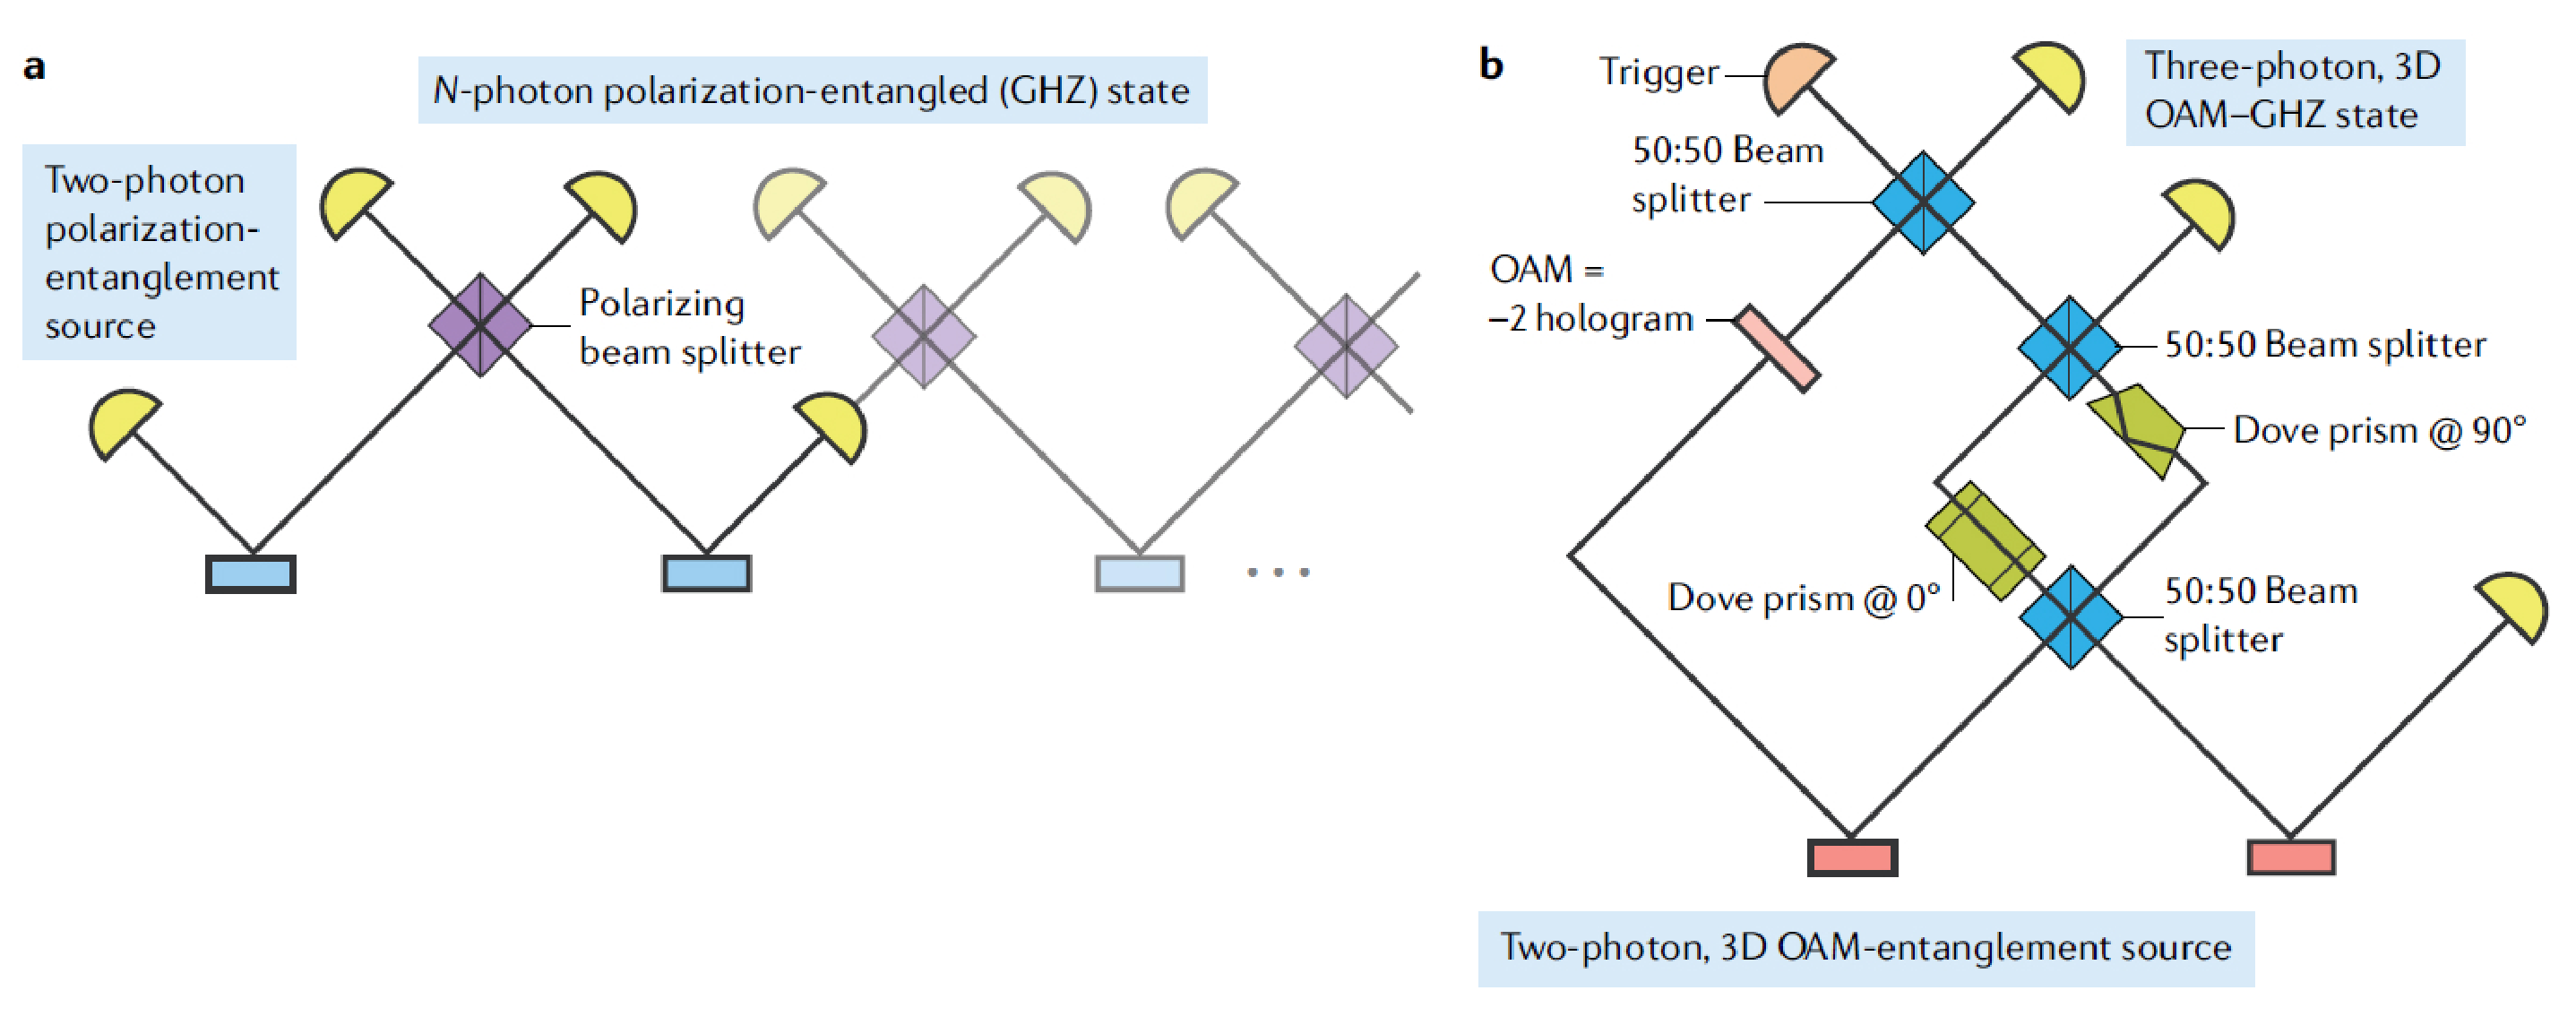
\includegraphics[width=\linewidth]{fig}
\caption{\textbf{Title.} a | Text. b | Text. c | Text. d | Text maximum 250 words. Panel a is adapted/reproduced with permission from ref.123, Springer Nature Limited. Panel b is adapted/reproduced with permission from ref.124, Publisher Name.}
\label{fig}
\end{figure}



\begin{table}[ht]
\centering
\begin{tabular}{|l|l|l|}
\hline
Particle & Mass & Charge \\
\hline
 \multicolumn{3}{|c|}{Charged particles}\\
\hline
Electron & $9.10938356(11)\times10^{-31}$ kg & $-1e$ \\
\hline
Proton & $1.672621898(21)\times10^{-27}$ kg & $+1e$ \\
\hline
 \multicolumn{3}{|c|}{Neutral particles}\\
\hline
Neutron & $1.674927471(21)\times10^{-27}$ kg & $0$ \\
\hline
\end{tabular}
\caption{\label{tab}Tables have titles but no captions are allowed. All symbols and acronyms used in a table should be defined in a footnote. Example: Here $e$ is the elementary charge.}
\end{table}


\section*{References} 

150–200 references are suggested. All referenced work should be accepted for publication or on recognized Archive databases. References should be given superscript numbers and cited sequentially according to where they appear in the main text, followed by those in the text boxes, figure captions and then tables (i.e. the order they appear in this template).
Journal abbreviation in italics, volume number in bold. If there are six or more authors for a reference, only the first author should be listed, followed by 'et al.'. Journal name abbreviations are followed by a full stop. Please include full page ranges. \\

\noindent Please do not cite web sites in the reference list — these should be listed separately, with the URLs in the Related Links section (see below).  If you are unsure if the website is a ‘Related link’ or should go in the ‘References’ section then identify if there is a publication date on the website.  If there is a publication date, it is likely that the item will be in the ‘References’ section.  If there is no publication date, it is likely that the item will be in the ‘Related Links’ section.\\

\noindent When citing a book, please indicate if you are citing a specific page range or chapter.  Otherwise, we presume that you are citing the entire book.  \\

\noindent \textbf{Highlighted references (optional)} Please select 5–-10 key references and provide a single sentence for each, highlighting the significance of the work.\\

\noindent\textbf{Acknowledgements}\\
E.g. Funding agencies.\\

\noindent\textbf{Author contributions}\\
Please describe the contributions made by each author.  Please use the initials of the individual author to explain these contributions.  These contributions are also required when you upload the files to our submission website.\\

\noindent\textbf{Competing interests}\\
Nature Journals require authors to declare any competing interests in relation to the work described. Information on this policy is available \href{http://www.nature.com/authors/policies/competing.html}{here}. \\



\noindent\textbf{Supplementary information (optional)}
If your article requires supplementary information, please include these files for peer-review. Please note that supplementary information will not be edited.


\end{document}